% Unofficial University of Cambridge Poster Template
% https://github.com/andiac/gemini-cam
% a fork of https://github.com/anishathalye/gemini
% also refer to https://github.com/k4rtik/uchicago-poster
\documentclass[final]{beamer}
\usepackage[orientation=portrait,size=a1,scale=1.0]{beamerposter}

% ====================
% Packages
% ====================
\usetheme{gemini}
\usecolortheme{nott}
\usepackage[T1]{fontenc}
\usepackage{lmodern}
\usepackage{graphicx,wrapfig,float}
\usepackage{booktabs}
\usepackage{tikz}
\usepackage{svg}
\usepackage{newunicodechar}
\usepackage{pgfplots}
\pgfplotsset{compat=1.14}
\usepackage{anyfontsize}

% ====================
% User's Packages
% ====================
\usepackage[english]{babel}
\usepackage{mathtools}
\usepackage{threeparttable}
\usepackage[ruled,vlined]{algorithm2e}
\usepackage{minted}

%%% bibliography
\usepackage{natbib}
\bibliographystyle{plainnat}

\DeclarePairedDelimiter\floor{\lfloor}{\rfloor}
\DeclareSymbolFont{yhlargesymbols}{OMX}{yhex}{m}{n}
\DeclareMathAccent{\yhwidehat}{\mathord}{yhlargesymbols}{"62}

\newcommand{\mono}[1]{\verb|#1|}
\newcommand{\ceil}[1]{\lceil {#1} \rceil}
\newcommand{\norm}[1]{\lvert\lvert {#1} \rvert\rvert_1}
\newcommand{\specialcell}[2][c]{%
\begin{tabular}[#1]{@{}c@{}}#2\end{tabular}}
\renewcommand\qedsymbol{\emph{QED}}

\newunicodechar{τ}{$\tau$}
\newlength{\sepwidth}
\newlength{\colwidth}
\setlength{\sepwidth}{0.025\paperwidth}
\setlength{\colwidth}{0.45\paperwidth}
\newcommand{\separatorcolumn}{\begin{column}{\sepwidth}\end{column}}


% ====================
% Lengths
% ====================

% If you have N columns, choose \sepwidth and \colwidth such that
% (N+1)*\sepwidth + N*\colwidth = \paperwidth

% ====================
% Title
% ====================

\title{2AMD15 - Big Data Management}

\author{
    Calli Evers \and 
    Sander Cauberg \and 
    Filippo Daniotti \and
    Klará Tauchmanová \and \\
    Horea Breazu \and
    Filipe 
        da Costa Quinta Goncalves 
    Sobrinho
}

\institute[shortinst]{ Eindhoven University of Technology }

% ====================
% Footer (optional)
% ====================

\footercontent{
  %\href{https://www.tue.nl/en/}{https://www.tue.nl/en/} \hfill
  \hfill 2AMD15 Poster Session,  March 31, 2023 \hfill
  %5600 MB Eindhoven, Netherlands
}
% (can be left out to remove footer)


% ====================
% Logo (optional)
% ====================

% use this to include logos on the left and/or right side of the header:
\logoright{\includesvg[width=10cm,keepaspectratio]{../assets/images/tue-logo.svg}}
\logoleft{\includesvg[width=10cm,keepaspectratio]{../assets/images/tue-logo.svg}}

% ====================
% Body
% ====================

\begin{document}


% Refer to https://github.com/k4rtik/uchicago-poster
% logo: https://www.cam.ac.uk/brand-resources/about-the-logo/logo-downloads
% \addtobeamertemplate{headline}{}
% {
%     \begin{tikzpicture}[remember picture,overlay]
%       \node [anchor=north west, inner sep=3cm] at ([xshift=-2.5cm,yshift=1.75cm]current page.north west)
%       {\includegraphics[height=7cm]{logos/unott-logo.eps}}; 
%     \end{tikzpicture}
% }

\begin{frame}[t]
\begin{columns}[t]
\separatorcolumn

\begin{column}{\colwidth}

    % \begin{block}{Question 2}
    
SQL query for Question 2:
\begin{center}
    \inputminted[]{sql}{../assets/code/q2.sql}
\end{center}
    
\begin{columns}
    \begin{column}{.45\linewidth}
        \textbf{Optimization techniques:}
        \begin{itemize}
            \item Fine-tuning the usage of partitions
            \item Broadcast <id, vector> map to reduce network consumption
            \item Usage of \mintinline{python}{numpy.ndarray}s with 16 bits integers
        \end{itemize}
    \end{column}
    \begin{column}{.45\linewidth}
        \begin{figure}[H]
            \centering
            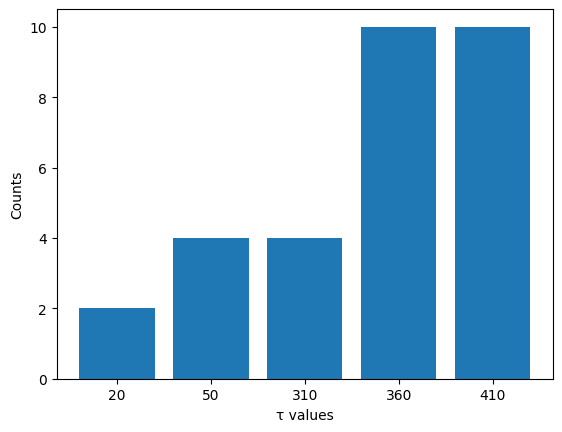
\includegraphics[width=.85\linewidth]{../assets/images/q2_results.png}
            \caption{Triples with aggregate variance $ \le \tau$}
            \label{fig:q2_results}
        \end{figure}
    \end{column}
\end{columns}

\begin{columns}
    \begin{column}{.45\linewidth}
        \begin{table}[H]
            \centering
            \begin{tabular}{l c}
    \toprule
    \textbf{Optimization} & \textbf{Execution time} \\
    \midrule
    All            & 163.56s    \\
    No numpy       & 443.19s    \\
    No repartition/coalesce  & 2108.38s     \\
    No broadcast   & ran out of heap    \\ 
    \bottomrule
\end{tabular}
\makeatletter\def\@captype{table}\makeatother% "Change float to table"
\caption{Impact of optimizations tricks on the dataset of size 125x10000, ran locally.}
\label{tab:q2_optimisations}
        \end{table}
    \end{column}
    \begin{column}{.45\linewidth}
        \begin{table}[H]
            \centering
            \begin{tabular}{l c}
    \toprule
    \textbf{Partitions} & \textbf{Execution time} \\
    \midrule
    32-64-128     & 237.11s    \\ 
    16-32-64      & 246.13s    \\ 
    64-128-256    & 295.03s    \\
    64-64-64      & 323.13s    \\
    \bottomrule
\end{tabular}
\makeatletter\def\@captype{table}\makeatother% "Change float to table"
\caption{Impact of partition combinations on the dataset of size 250x10000, ran on the server.}
\label{tab:q2_partitions}
        \end{table}
    \end{column}
\end{columns}
    
\end{block}

  
    % \begin{block}{Question 3}

System architecture for Question 3:

\begin{figure}[!h]
    \centering
    
\includegraphics[width=.95\linewidth]{../assets/images/q3_diagram.png}
    \caption{Brief description of system architecture for Q3}
    \label{fig:q3_diagram}
\end{figure}

\textbf{Optimization techniques:}

\begin{itemize}
    \item Fine-tuning the usage of partitions
    \item Broadcast <id, vector> map to reduce network consumption
    \item Usage of \mintinline{python}{numpy.ndarray}s with 16 bits integers
    \item Usage of \mintinline{python}{.Accumulator()} API 
    \item Caching filtered triples with $var \le 410$ before filtering again for $var \le 20$ \emph{(discarded)}
    \item Pre-computing the mean of each vector to speed up \mintinline{python}{statistics.pvariance()} \emph{(discarded)}
\end{itemize}

\begin{columns}
    \begin{column}{.5\textwidth}
        \begin{table}[!h]
            \centering
            \begin{tabular}{l c}
    \toprule
    \textbf{Optimization} & \textbf{Execution time} \\
    \midrule
    All            & 30.59s     \\
    No numpy       & 2940.19s   \\
    No broadcast   & 185.30s    \\ 
    No accumulator & 36.44s     \\
    No coalesce    & 131.46s    \\
    \bottomrule
\end{tabular}
\caption{Impact of optimizations tricks on the dataset of size 250x10000, ran locally.}
\label{tab:q3_local_optimisations}
        \end{table}
    \end{column}
    
    \begin{column}{.5\textwidth}
        \begin{table}[!h]
            \centering
            \begin{tabular}{l c}
    \toprule
    \textbf{Partitions} & \textbf{Execution time} \\
    \midrule
    64-128-256     & 910.05s    \\ 
    128-256-512    & 946.79s    \\ 
    125-250-500    & 969.51s    \\ 
    64-64-128      & 1005.65s   \\
    25-50-100      & 1097.70s   \\
    64-64-64       & 1122.74s   \\
    128-128-128    & 1162.01s   \\
    \bottomrule
\end{tabular}
\caption{Impact of partition combinations on the dataset of size 1000x10000, ran on the server.}
\label{tab:q3_server_optimisations}
        \end{table}
    \end{column}
\end{columns}
    
\end{block}
    % \begin{block}{Question 2 vs. Question 3}
    Both solution produced the \textbf{same results}:
    \begin{table}[H]
        \centering
        \begin{tabular}{l r r c}
    \toprule
    {} & \textbf{Q2 code} & \textbf{Q3 code} \\
    \midrule
    Results $\tau = 20$ & 2
    % 2%, [ARSR-JIIT-JY1T], [CFIL-D4U2-OE4G] 
    & 10  \\
    Results $\tau = 420$ & 2%, [ARSR-JIIT-JY1T], [CFIL-D4U2-OE4G]
    & 10  \\
    \midrule
    Execution time & 237.11 & 42.35&  \\
    \bottomrule
\end{tabular}
\makeatletter\def\@captype{table}\makeatother% "Change float to table"
\caption{Comparison between Q2 code and Q3 code on the same dataset (250 vectors).}
\label{tab:q2-vs-q3}
    \end{table}
    % Tests were performed running the code of Question 3 on the data generated for Question 2.  Even though the differences in the implementation of Q3 are not so trivial the main differences are as follows:
    % \begin{itemize}
    %     \item A different use of the \mintinline{python}{.coalesce()} and \mintinline{python}{.repartition()}
    %     \item A different number of queries. Q3 only queries two values (\(\tau \le 20\) and \(\tau \le 410\)) compared to 5 for Q2.
    %     \item The \mintinline{python}{DataFrame} API of Spark SQL might be inherently slower than the usage of plain Spark.
    % \end{itemize}
    
\end{block}
    % \begin{block}{References}

\bibliography{references}

\end{block}

\end{column}

\separatorcolumn

\begin{column}{\colwidth}

    %  \begin{block}{Question 4}
We used \textbf{Count-min (CM) sketch} (\cite{cm-sketch}). Illustration of the approximation of the aggregate variance:

\begin{figure}
    \centering
    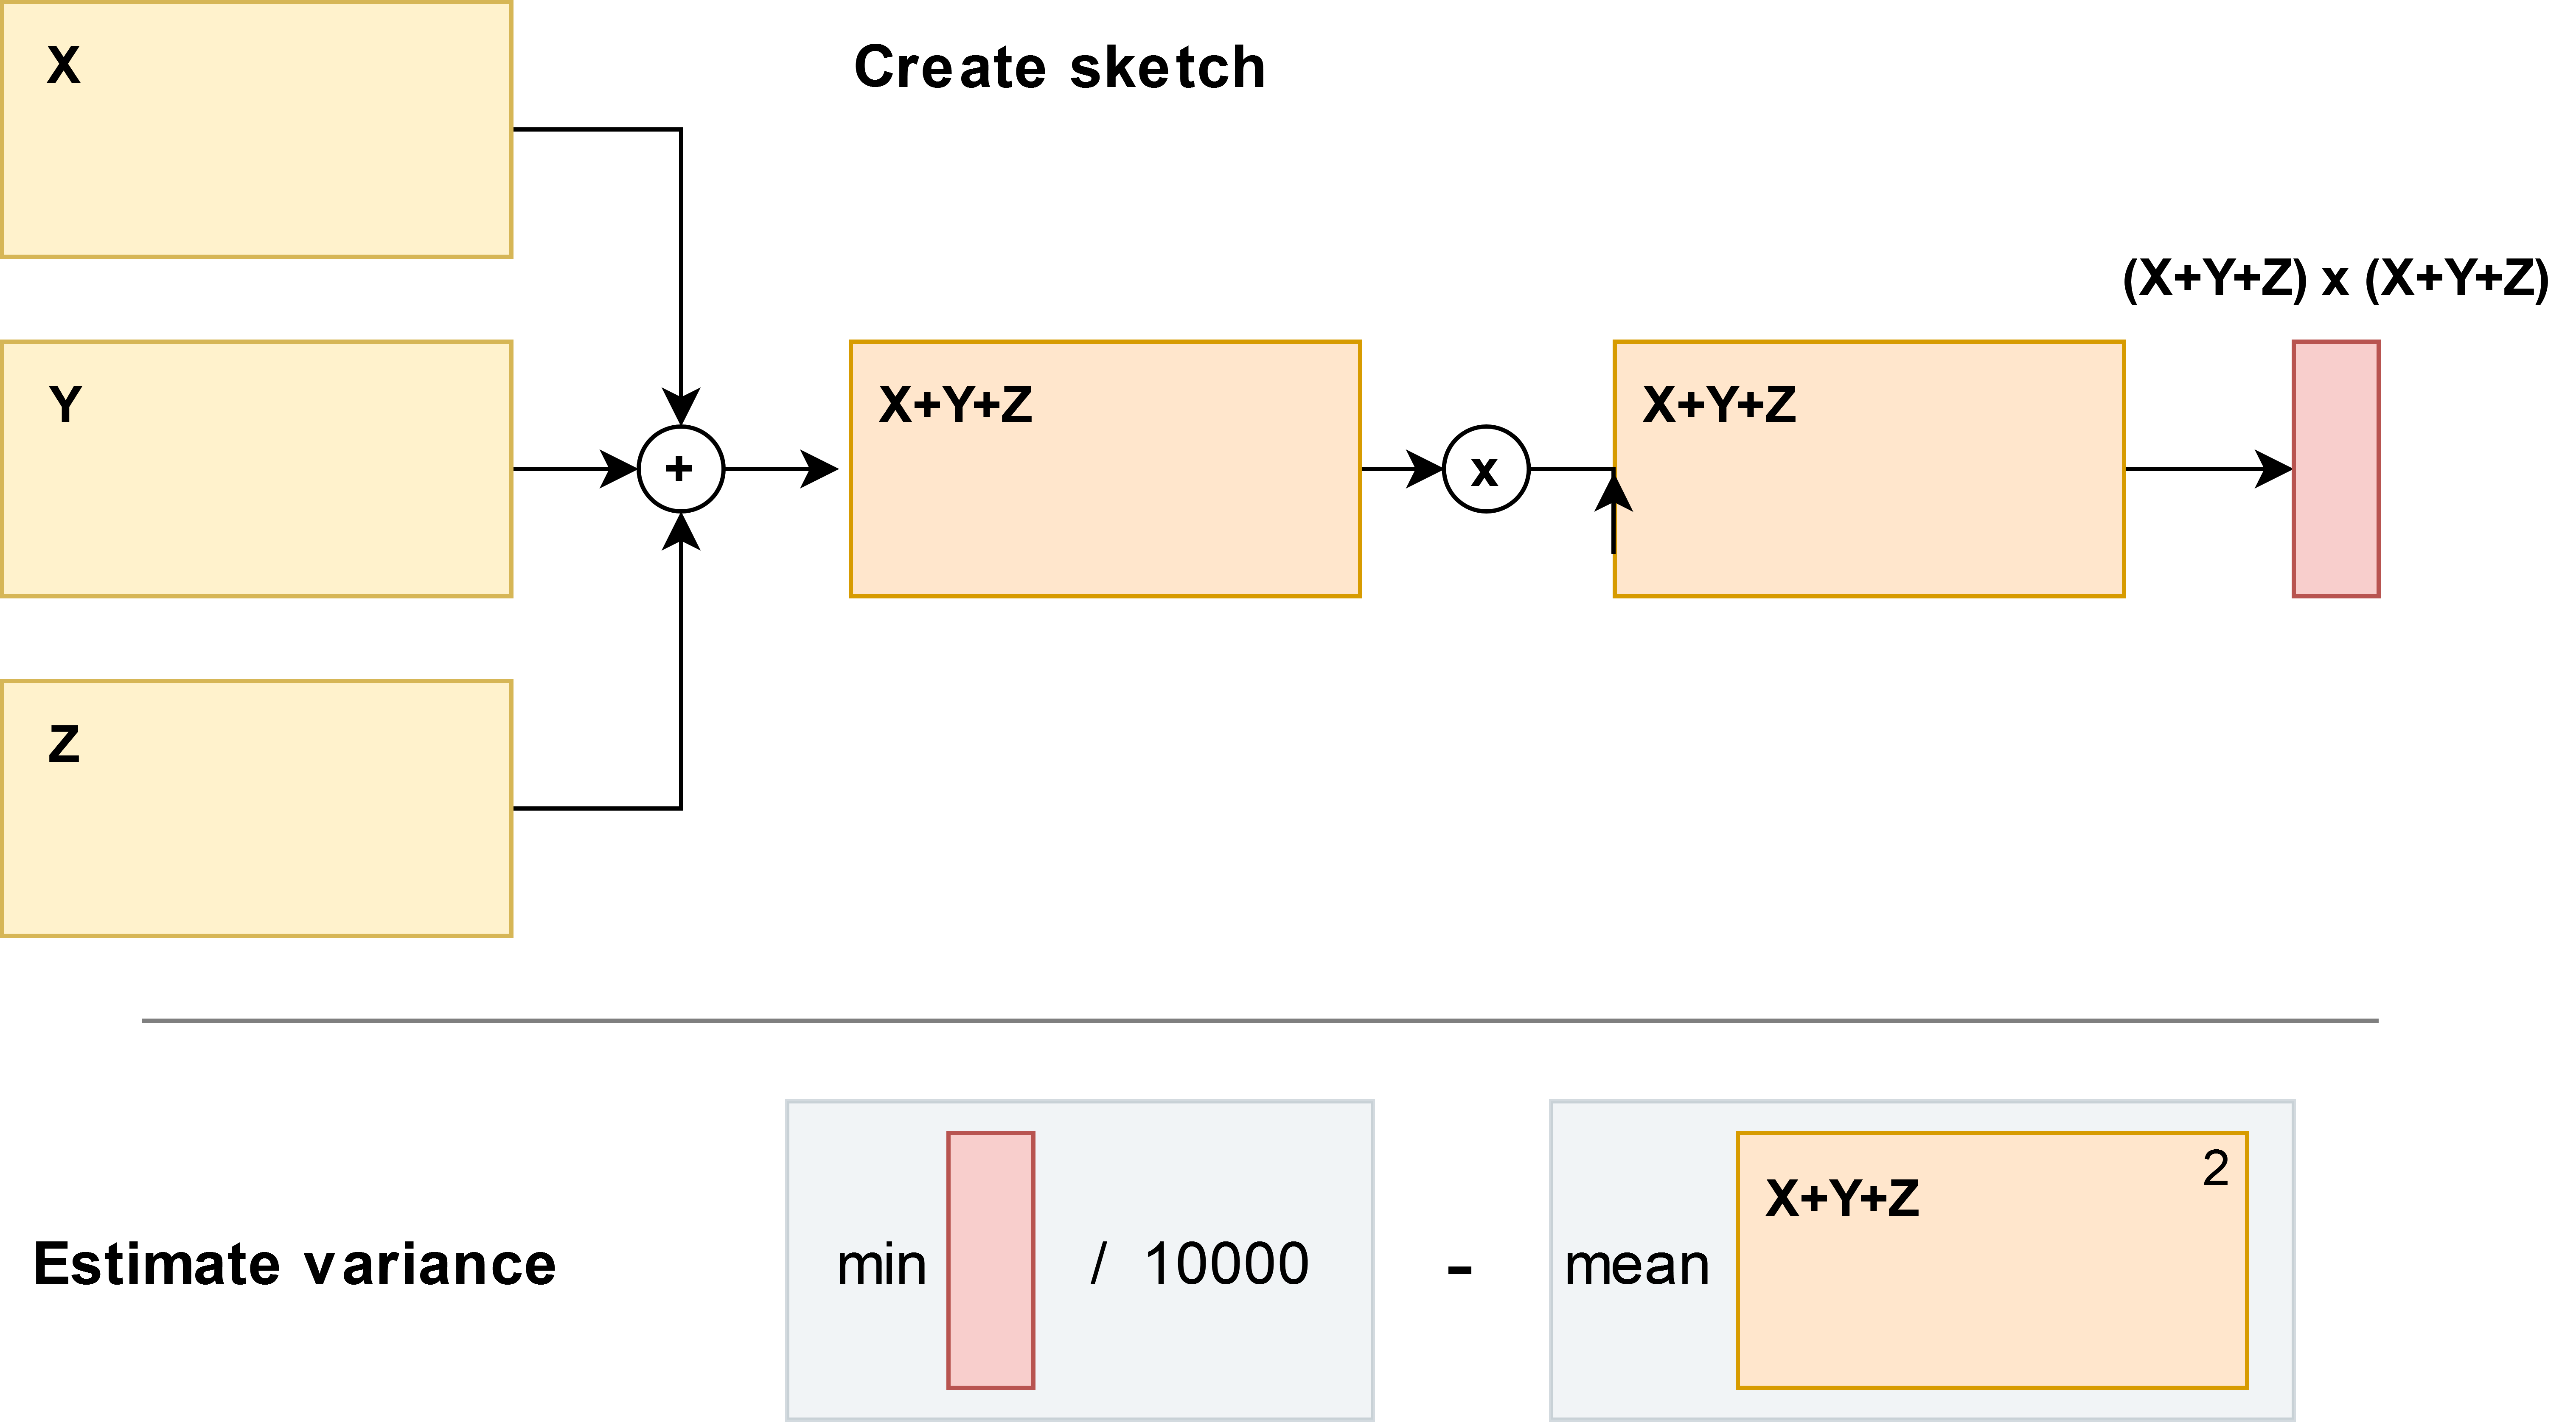
\includegraphics[width=.8\linewidth]{../assets/images/q4_sketch_usage.png}
    \caption{Count-min sketch exploitation for Q4}
    \label{fig:q4_sketch}
\end{figure}

%Formally, the approximated aggregate variance can be expressed as follows,
%\begin{equation}
%    \widehat{\sigma}^2=\left(\frac{1}{10000}\widehat{(\mathbf{a}\odot\mathbf{a})}\right)-\mu_{\mathbf{a}}^2
%\end{equation}

% \begin{columns}[t]
%    \begin{column}{.5\textwidth}
%        \begin{algorithm}[H]
    \label{alg:create_sketch}    
    \caption{Creates CM sketch from vector.}
    \DontPrintSemicolon
    
    \KwIn{vector[], hash\_functions, $\varepsilon$, $\delta$}
    \KwOut{sketch[]}
    \;        
    $w$ = $\ceil{e / \varepsilon}$,
    $d$ = $\ceil{\ln 1 / \delta}$\;
    sketch[] = new Table(size = ($w$, $d$), fill = $0$)\;
    \For {$i = 0$ to  $10000$}{
        \For{$j = 0$ to $d$}{
            index = hash\_functions~$[j](i)$ mod $w$\;
            sketch[$j$, index] $\leftarrow$ sketch[$j$, index] + vector[$i$]
        }
    }
    \Return sketch
        
\end{algorithm}

%    \end{column}
%    \hfill
%    \begin{column}{.5\textwidth}
%        \begin{algorithm}[H]
    \label{alg:merge_and_variance}
    \caption{Computes aggregate variance.}
    \DontPrintSemicolon

    \KwIn{sketch\_1, sketch\_2, sketch\_3, $w$}
    \KwOut{approx\_agg\_var}
    \;
    approx\_agg\_var = sketch\_1 + sketch\_2 + sketch\_3\;
    % \inner = \skAgg $\odot$ \skAgg\;
    inner\_product = $\sum_{j=1}^{w}$ (approx\_agg\_var$[j]^2$)\;
    
    \Return $\frac{1}{10000}$min(inner\_product) $-$ $\mu^2_{\textrm{inner\_product}}$

\end{algorithm}
%        \vspace{0pt}
%    \end{column}
% \end{columns}

\textbf{Theorem 1.} $\sigma^2\leq\widehat{\sigma^2}$ and, with probability $1-\delta$, we have that $\widehat{\sigma^2}\leq\sigma^2 + \frac{1}{10000}\varepsilon\norm{\mathbf{a}}^2$

\emph{Proof.} By the definition of $\widehat{\sigma^2}$ and $\sigma^2$ and from the \textbf{Theorem 3} from the \cite{cm-sketch} paper
\begin{equation}
    \sigma^2=\frac{1}{10000}(\mathbf{a}\odot\mathbf{a})-\mu_{\mathbf{a}}^2\leq\frac{1}{10000}\widehat{(\mathbf{a}\odot\mathbf{a})}-\mu_{\mathbf{a}}^2=\widehat{\sigma^2}    
\end{equation}

Therefore, $\sigma^2\leq\widehat{\sigma^2}$ for non-negative vectors. Similarly,
\begin{equation}
    \begin{aligned}
    \mathbb{P}\left[\widehat{\sigma^2} - \sigma^2 \geq \frac{1}{10000}\varepsilon\norm{\mathbf{a}}^2\right] & = \mathbb{P}\left[\frac{1}{10000}\left(\widehat{(\mathbf{a}\odot\mathbf{a})} - (\mathbf{a}\odot\mathbf{a})\right) \geq \frac{\varepsilon\norm{\mathbf{a}}^2}{10000}\right] \\ 
    & = \mathbb{P}\left[\left(\widehat{(\mathbf{a}\odot\mathbf{a})} - (\mathbf{a}\odot\mathbf{a})\right) \geq \varepsilon\norm{\mathbf{a}}^2\right]\leq\delta
    \end{aligned}
\end{equation}

So, $\mathbb{P}\left[\widehat{\sigma^2} - \sigma^2 \geq \frac{1}{10000}\varepsilon\norm{\mathbf{a}}^2\right]\leq\delta$, as required.
\begin{flushright}
    \emph{QED}
\end{flushright}

System architecture for Question 4:
\begin{figure}
    \centering
    
\includegraphics[width=.95\linewidth]{../assets/images/q4_diagram.png}
    \caption{Brief description of the system architecture for Q4}
    \label{fig:q4_diagram}
\end{figure}

The execution time of Q4 on the cluster: \textbf{164.33 seconds} 

\begin{center}
    \begin{threeparttable}[b]
    \begin{tabular}{c | c c c c}
        \toprule
        \textbf{} & \textbf{$\epsilon=0.0001$} & \textbf{$\epsilon=0.001$} & \textbf{$\epsilon=0.002$} & \textbf{$\epsilon=0.01$} \\
        \midrule
        \textbf{$\tau \leq 400$} & - & $P=1\tnote{1},R=0/10$ & - & $P=1\tnote{1},R=0/10$ \\
        \textbf{$\tau \geq 200000$} & $P=1,R=1$ & $P=1/26819,R=1$ & $P=1/91885,R=1$ & $P=1/2573000,R=1$ \\
        \textbf{$\tau \geq 1000000$} & $P=1\tnote{1},R=1\tnote{2}$ & $P=1\tnote{1},R=1\tnote{2}$ & $P=0/1,R=1\tnote{2}$ & $P=0/91885,R=1\tnote{2}$ \\
        \bottomrule
    \end{tabular}
    \begin{tablenotes}
            \item [1] Number of TPs is 0, number of FTs is also 0 (eg. 0/0)
            \item [2] Number of relevant triplets is 0, number of retrieved triplets is also 0 (eg. 0/0)
       \end{tablenotes}
\caption{Precision/recall values of the Q4 results.}
\label{tab:q4-precision-recall}
\end{threeparttable}
\end{center}

\emph{CM sketch} always \textbf{overestimating} the results, therefore:
\begin{itemize}
    \item for \emph{functionality 1} ($\leq\tau$): counts are underestimated, only TP triplets $\rightarrow$ precision is 1
    \item for \emph{functionality 2} ($\geq\tau$): counts are overestimated, lots of FP triplets, but no FNs $\rightarrow$ recall is 1
    \item smaller $\delta$ $\rightarrow$ larger depth $d$ $\rightarrow$ a better approximation of the aggregate variance $\rightarrow$ higher recall for \emph{functionality 1} and higher precision for \emph{functionality 2}
    \item for smaller $\varepsilon$ $\rightarrow$ larger width $w$ $\rightarrow$ fewer collisions $\rightarrow$ a better approximation $\rightarrow$ higher recall for \emph{functionality 1} and higher precision for \emph{functionality 2}
\end{itemize}

The dimension of the sketch is important:
\begin{itemize}
    \item too small $\varepsilon$ $\rightarrow$ huge size of the sketch $\rightarrow$ slow computation, but more precise results
    \item too big $\varepsilon$ $\rightarrow$ small size of the sketch $\rightarrow$ fast computation, but high number of FPs 
\end{itemize}

The tightness of the bounds:
\begin{itemize}
    \item \emph{lower bound}: tight
    \item \emph{upper bound}: vary for each aggregate vector, the error is relative to the first norm squared
\end{itemize}
    
\end{block}
    % \begin{block}{Ethical and other aspects}

% Depending on the actual size of the company, our employed technique would differ. From our tests we've seen that these types of computing problems are memory and CPU dependent. Furthermore, due to security constraints we avoid any cloud hosting clusters. Taking these into account, we chose the following two options:

% \begin{itemize}
%     \item\textbf{c)} Spark, on a company owned server. We consider this strategy, because we've seen that Spark can be easily scaled and programmed with both Java and Python APIs.
%     \item\textbf{e)} An approximation technique, similar to the solution of Q4, but running on a powerful server. In this situation the most important parameters that we have to look for are $\epsilon$ and $\delta$. If by "powerful server" it means that there are no restrictions on the CPU and memory usage, then $\epsilon$ and $\delta$ should be asymptotically small thus generating higher precision and recall for the employed sketches.
% \end{itemize}

% In order to decide the appropriate technique, we would consider the following:
% \begin{enumerate}
%     \item size of the problem
%     \item precision/recall requirements of the company
%     \item hardware availability of the company
%     \item sensitivity of the data/context
% \end{enumerate}

\begin{itemize}
    \item \emph{Relational databases} should be employed if the size of the problem is small, because:
    \begin{itemize}
        \item they are more widely known (thus maintainable)
        \item no need to add complexity if the problem is small
    \end{itemize}
    \item \emph{Multi-threaded programs} should be avoided, because:
    \begin{itemize}
        \item it does not provide developers with any advantage over Spark
        \item Spark provides users with better scalability
    \end{itemize}
    \item \emph{Company-owned cluster vs. cloud resources} - the choice is a trade-off between:
    \begin{itemize}
        \item hardware/resources availability of the company
        \item sensitivity of the data/context
    \end{itemize}
    \item \emph{Spark vs. approximation technique} - the choice depends on:
    \begin{itemize}
        \item hardware/resources availability of the company
        \item precision/recall requirements of the company for the problem
    \end{itemize}
\end{itemize}

\end{block}

\end{column}
\separatorcolumn

\end{columns}
\end{frame}

\end{document}
